\documentclass[10pt,a4paper]{article}
\usepackage[utf8]{inputenc}
\usepackage[T1]{fontenc}
\usepackage{lmodern}
\usepackage{babel}
\babelprovide[import,main]{french}
\usepackage[margin=1.7cm,top=1.4cm,bottom=1.3cm]{geometry}
\usepackage{graphicx,booktabs,hyperref,microtype}
\usepackage{titlesec}
\pagestyle{empty}
\setlength{\parindent}{0pt}\setlength{\parskip}{3pt}
\titleformat{\section}{\large\bfseries}{}{0em}{}
\titlespacing*{\section}{0pt}{6pt}{2pt}
\begin{document}
{\LARGE\bfseries Numériseur 4~voies à 250~Mech/s : étude préliminaire de la numérisation et du déclenchement configurable}\\[2pt]
{\small Douaa Guermassi --- simulation Python et Verilog vérifié (Icarus Verilog) ; code : github.com/douaa-g}

\section{Objectif}
La proposition de stage « Développement d'un numériseur configurable » (LPSC, service électronique) vise une carte à quatre voies numérisées à 250~Mech/s, avec des équations de déclenchement définies par l'utilisateur, un oscillogramme, des histogrammes d'amplitude et de différences de temps entre voies. Pour me familiariser avec ce domaine, j'ai étudié sur des impulsions simulées deux questions : (1) quelle résolution temporelle reste possible quand on échantillonne toutes les 4~ns, et que change la bande passante d'entrée ? (2) comment réaliser un déclenchement par équations dont la modification ne demande pas de nouvelle synthèse, idée que j'ai retrouvée dans les modules UCTM/UCTM2 de l'équipe (arXiv:1603.06816) ? Il s'agit d'une étude de \emph{principe} : les impulsions sont illustratives (montée 2~ns, descente 20~ns), pas celles de vos détecteurs. Elle prolonge mon étude du discriminateur à fraction constante (CFD) numérique (github.com/douaa-g/CFD-timing-study).

\section{Résolution temporelle à 250~Mech/s}
Chaque impulsion est générée sur une grille fine (16~GS/s), filtrée par un passe-bas du 2\textsuperscript{e} ordre (étage d'entrée, fréquence de coupure $f_c$), échantillonnée à 250~Mech/s avec une phase d'arrivée aléatoire, puis un bruit blanc est ajouté (SNR~=~100). Le temps est obtenu par CFD numérique ($y[n]=f\,x[n]-x[n-d]$, passage par zéro) avec interpolation linéaire ou cubique (4~points). Les paramètres $(f,d)$ sont choisis sur un jeu d'événements et évalués sur un jeu indépendant (3\,000 événements chacun).

\begin{minipage}[t]{0.52\linewidth}\vspace{0pt}\centering
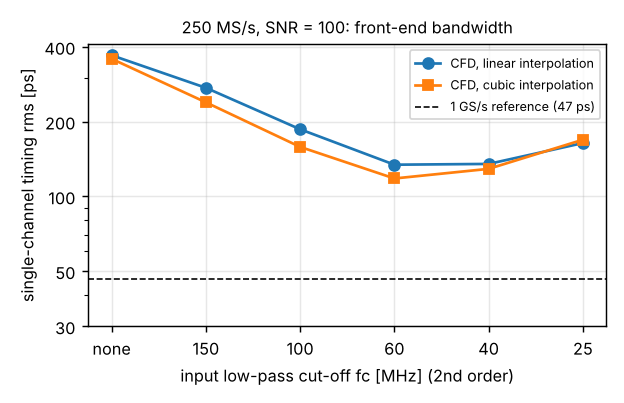
\includegraphics[width=\linewidth]{figures/fig_frontend.png}
\end{minipage}\hfill
\begin{minipage}[t]{0.45\linewidth}\vspace{4pt}
\begin{itemize}\setlength{\itemsep}{1pt}\setlength{\leftmargin}{8pt}
\item Sans filtre d'entrée, la résolution est de 370~ps par voie (à comparer à 47~ps à 1~GS/s) : le pas de 4~ns est comparable au temps de montée.
\item Avec $f_c=60$~MHz, elle tombe à 134~ps (interpolation linéaire) et 118~ps (cubique, soit 12\,\% de mieux). Le choix de la bande passante pèse donc plus que celui de l'algorithme.
\item Plus bas ($f_c=25$~MHz), la montée devient trop lente et la résolution se dégrade à nouveau (164--169~ps) : il existe un optimum, ici autour de 60~MHz.
\end{itemize}
\end{minipage}

\section{Chaîne 4 voies et déclenchement par équations}
\textbf{Architecture (Verilog).} Quatre CFD en virgule fixe (12~bits, $f=5/8$, $d=3$~échantillons) alimentent un bloc de déclenchement : le premier impact ouvre une porte, les impacts arrivant dans les \texttt{WIN} cycles suivants sont accumulés, puis une table de vérité de 16~entrées (indexée par $\{D,C,B,A\}$) décide du déclenchement. Décider une seule fois par porte permet les vétos et le OU exclusif ; le prix est une latence fixe (24~ns ici). Des compteurs 32~bits comptent les impacts et les déclenchements. Un compilateur Python transforme une équation texte (par ex. \texttt{(A \& B) \& !D}, \texttt{MULT(2, A, B, C, D)}) en table de vérité chargée par une interface de registres : changer d'équation ne change pas le firmware.

\textbf{Vérification.} Un flux de 160~$\mu$s (40\,000 échantillons par voie) contient 162 événements de topologies connues (quelles voies, temps d'arrivée à $\pm 6$~ns, amplitudes), soit 349 impulsions. Les quatre CFD ont produit 349 impacts, sans impact parasite ni manquant. Pour sept équations, les sorties du RTL (impacts, déclenchements, compteurs) sont identiques bit à bit à un modèle Python cycle par cycle, et le nombre de déclenchements égale celui attendu d'après les topologies injectées (par ex. \texttt{A \& B \& C} : 40 attendus, 40 obtenus). Un test négatif (mauvaise table ou mauvaise porte dans le modèle) fait bien échouer la comparaison.

\textbf{Interface Qt.} Une interface PySide6 (Qt pour Python) permet de saisir l'équation (compilation en direct, message d'erreur), de régler la porte, de lire les compteurs, de passer d'un déclenchement à l'autre sur l'oscillogramme, et d'afficher les histogrammes d'amplitude et de différences de temps, au choix pour tous les impacts ou seulement ceux des portes ayant déclenché. Elle utilise les modèles vérifiés contre le Verilog et redonne les mêmes décomptes pour les sept équations (test scripté).

\begin{center}
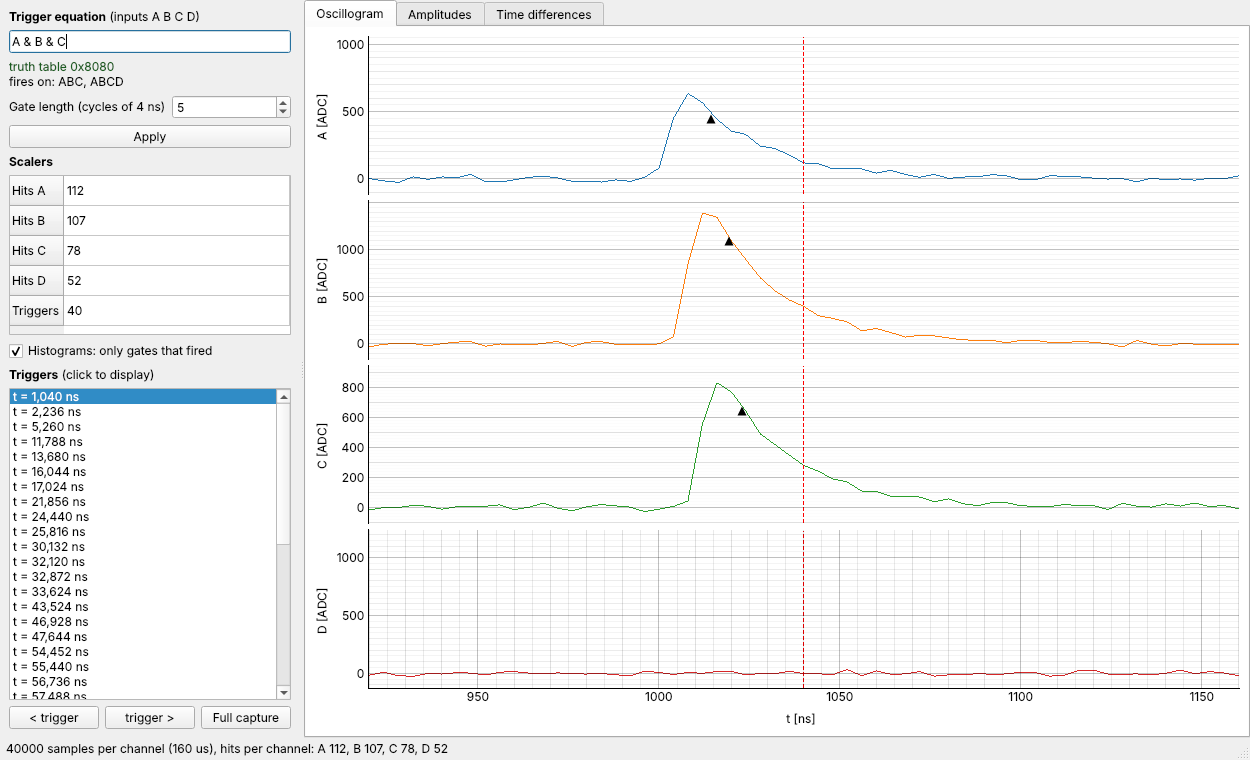
\includegraphics[width=0.8\linewidth]{figures/qt_osc.png}
\end{center}

\begin{center}
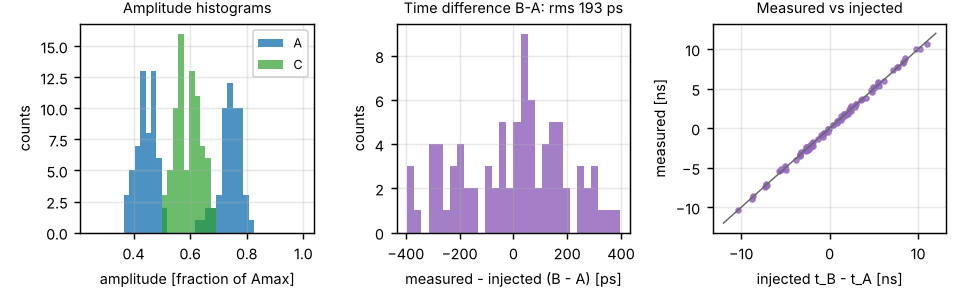
\includegraphics[width=0.8\linewidth]{figures/fig_viewer_hist.png}
\end{center}

\begin{minipage}[t]{0.56\linewidth}\vspace{0pt}\centering
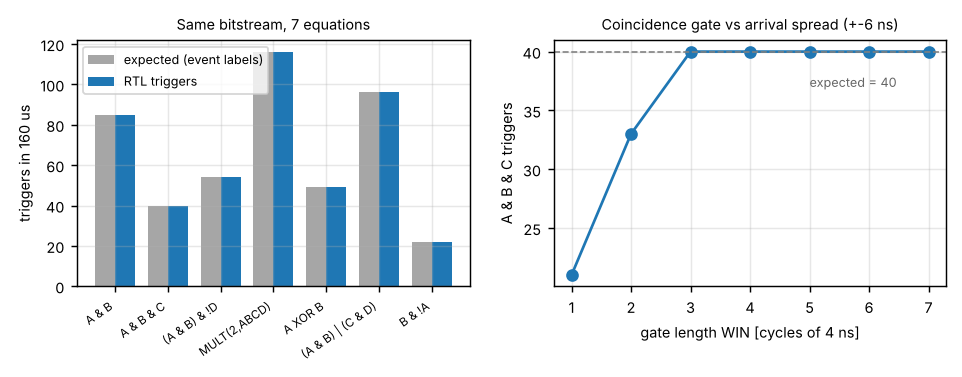
\includegraphics[width=\linewidth]{figures/fig_trigger.png}
\end{minipage}\hfill
\begin{minipage}[t]{0.41\linewidth}\vspace{2pt}
\begin{itemize}\setlength{\itemsep}{1pt}\setlength{\leftmargin}{8pt}
\item \textbf{Porte :} avec des arrivées étalées sur $\pm 6$~ns, il faut au moins 3~cycles ; en dessous, des coïncidences sont perdues (21 sur 40 avec un cycle).
\item \textbf{Différence de temps $B-A$ :} 85~coïncidences, écart-type 193~ps, cohérent avec $\sqrt{2}\times 134$~ps $\approx 190$~ps.
\end{itemize}
\end{minipage}

\section{Limites et questions}
Impulsions illustratives, bruit blanc, mêmes réglages sur les quatre voies, pas de défauts du CAN (non-linéarités, gigue d'horloge), interpolation faite en logiciel, RTL comportemental simulé sous Icarus (ni synthèse ni analyse de timing), Les chiffres ne sont donc pas ceux d'une carte réelle. Ce que j'aimerais comprendre avec vous : la bande passante et la résolution réelles de l'étage d'entrée et du CAN prévus, les formes d'impulsions des détecteurs visés, et la latence de déclenchement tolérable.
\end{document}
